% ============================================================================
% chapitre3.tex — Conception
% ============================================================================
\chapter{Conception}
\label{chap:conception}

\introchapitre

Ce chapitre presente la conception du systeme. Nous abordons successivement la
modelisation dynamique (sequence, etats-transitions, activite), la modelisation
statique (classes, modele relationnel, dictionnaire de donnees) et l'architecture
generale de l'application (composants, deploiement).

\section{Modelisation dynamique}
\label{sec:dynamique}

\subsection{Diagramme de sequence}

Le diagramme de sequence illustre le flux dynamique d'une transaction de paiement a
travers les quatre jobs Flink successifs, depuis sa publication par le producteur
jusqu'a sa persistance finale dans PostgreSQL.

\textbf{Description des participants :}
\begin{itemize}
    \item \textbf{Producer} : publie les transactions chiffrees (payload Fernet) dans
    le topic \texttt{payments},
    \item \textbf{Kafka Broker} : stocke et route les messages entre les jobs via les
    topics du pipeline,
    \item \textbf{Job 1 --- Decryption} : dechiffre le payload Fernet et ecrit
    l'enregistrement brut dans la couche Bronze de MinIO,
    \item \textbf{Job 2 --- Validation} : applique les 9 regles de validation et route
    les transactions invalides vers la DLQ,
    \item \textbf{Job 3 --- Normalisation} : convertit les dates en ISO 8601, normalise
    les montants et enrichit les donnees ISO,
    \item \textbf{Job 4 --- Optimisation} : deduplique par \texttt{AUTHORIZATION\_CODE},
    calcule le score de risque et publie vers \texttt{payments.gold},
    \item \textbf{gold-flattener / Kafka Connect} : republie l'enregistrement sous
    forme de message a schema explicite, puis l'insere dans \texttt{gold\_transactions}
    via le connecteur JDBC Sink.
\end{itemize}

\textbf{Fragments \texttt{alt} :} si le decryptage echoue (\texttt{INVALID\_FERNET\_TOKEN}),
le message est route vers \texttt{payments.dlq} ; si une des 9 regles de validation
echoue, un \texttt{rejectReason} machine-readable est ajoute et le message est route
vers la DLQ ; sinon, la transaction est normalisee, enrichie, dedupliquee, puis
publiee dans \texttt{payments.gold} avant d'etre inseree dans
\texttt{gold\_transactions} via un \textit{upsert}.

\begin{figure}[H]
\centering
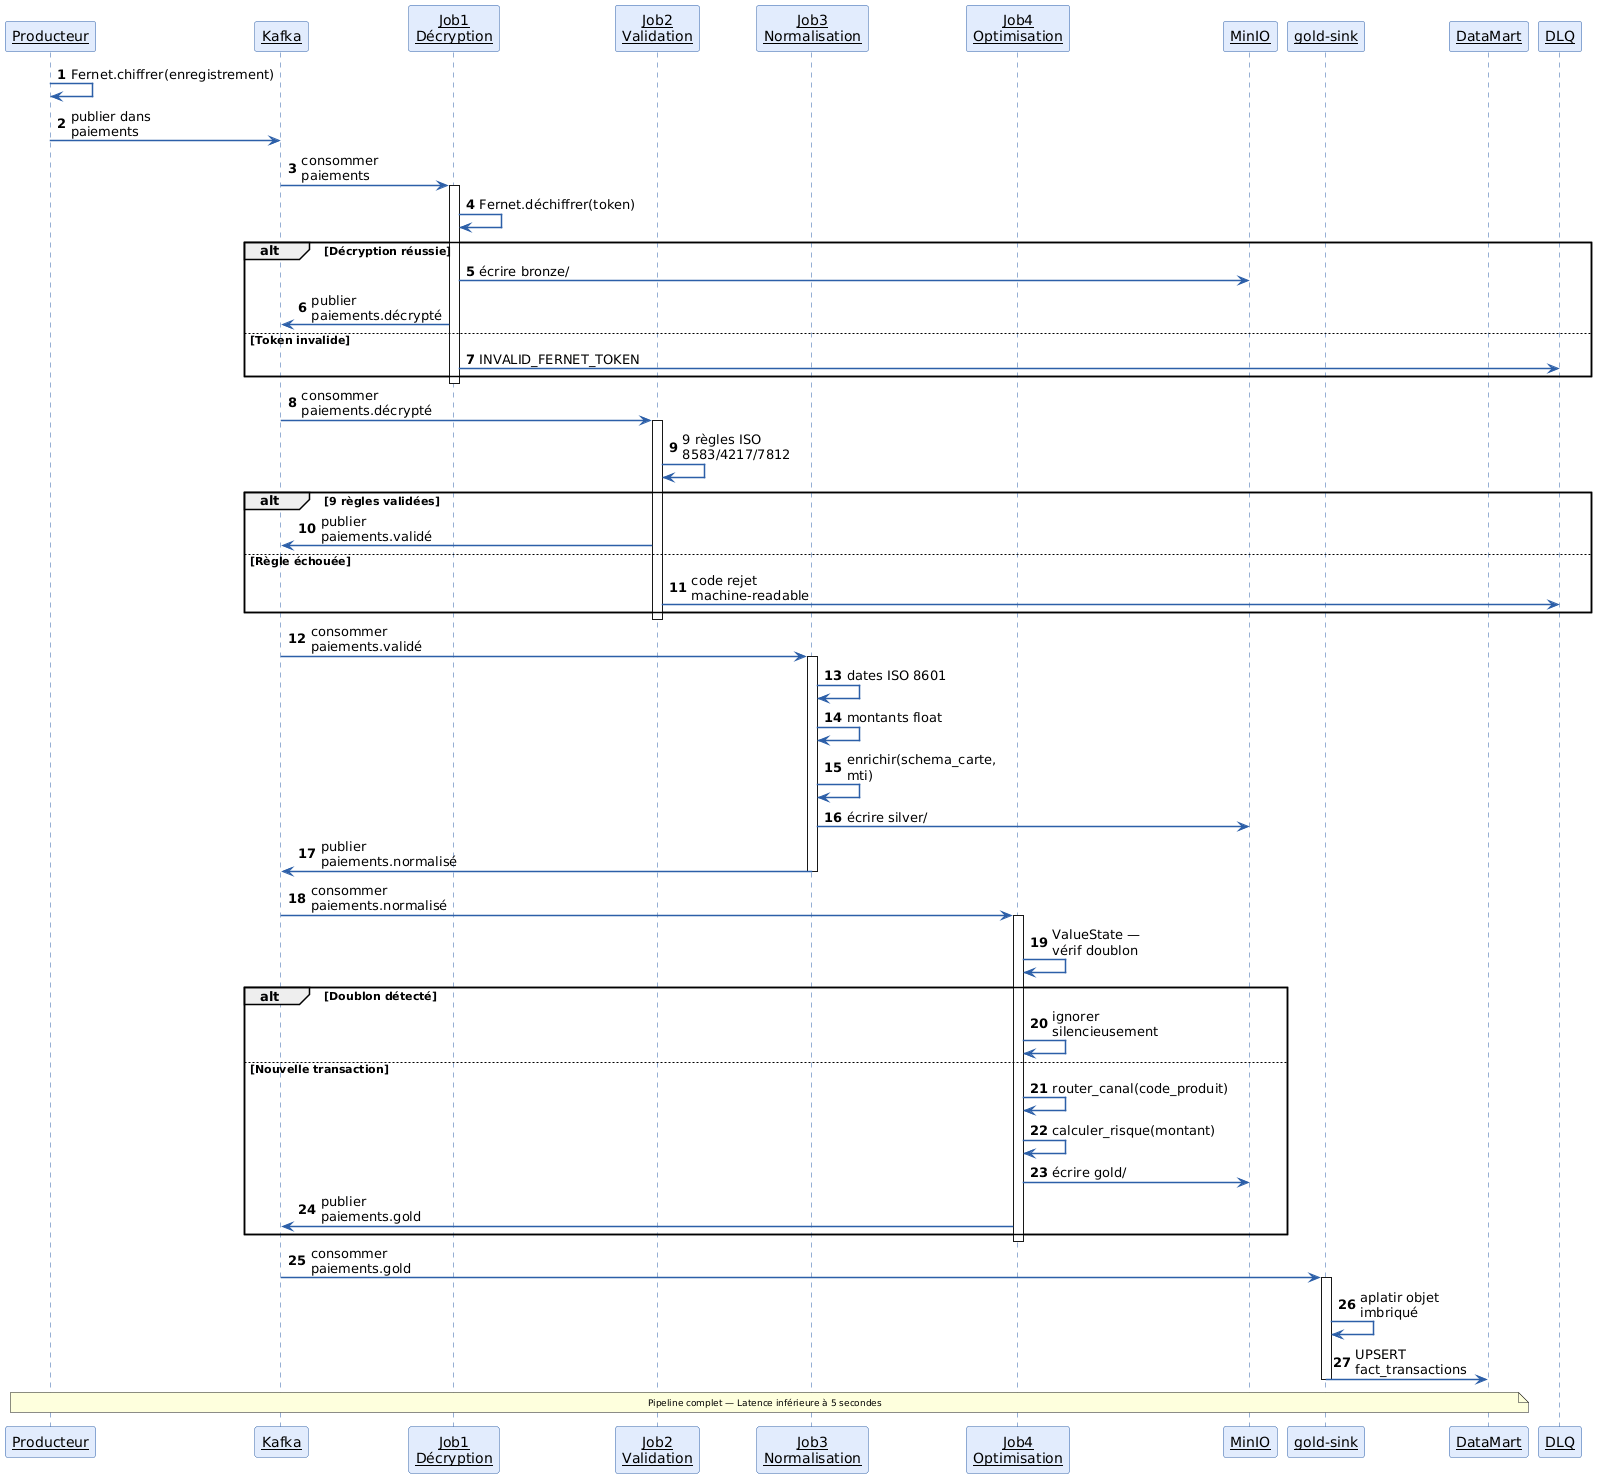
\includegraphics[width=\textwidth]{figures/sequence.png}
\caption{Diagramme de sequence --- traitement d'une transaction a travers le pipeline}
\label{fig:sequence}
\end{figure}

\subsection{Diagramme d'etats-transitions}

Le diagramme d'etats-transitions (figure \ref{fig:etats}) modelise le cycle de vie
d'une transaction a travers neuf etats successifs : \textit{Produit}, \textit{Chiffre},
\textit{Publie}, \textit{Decrypte}, \textit{Valide}, \textit{Normalise},
\textit{Optimise}, \textit{Synchronise} (etat final nominal) et \textit{Rejete} (etat
final d'erreur, atteignable depuis les etats \textit{Publie} et \textit{Decrypte} en
cas de token invalide ou de regle de validation echouee).

\begin{figure}[H]
\centering
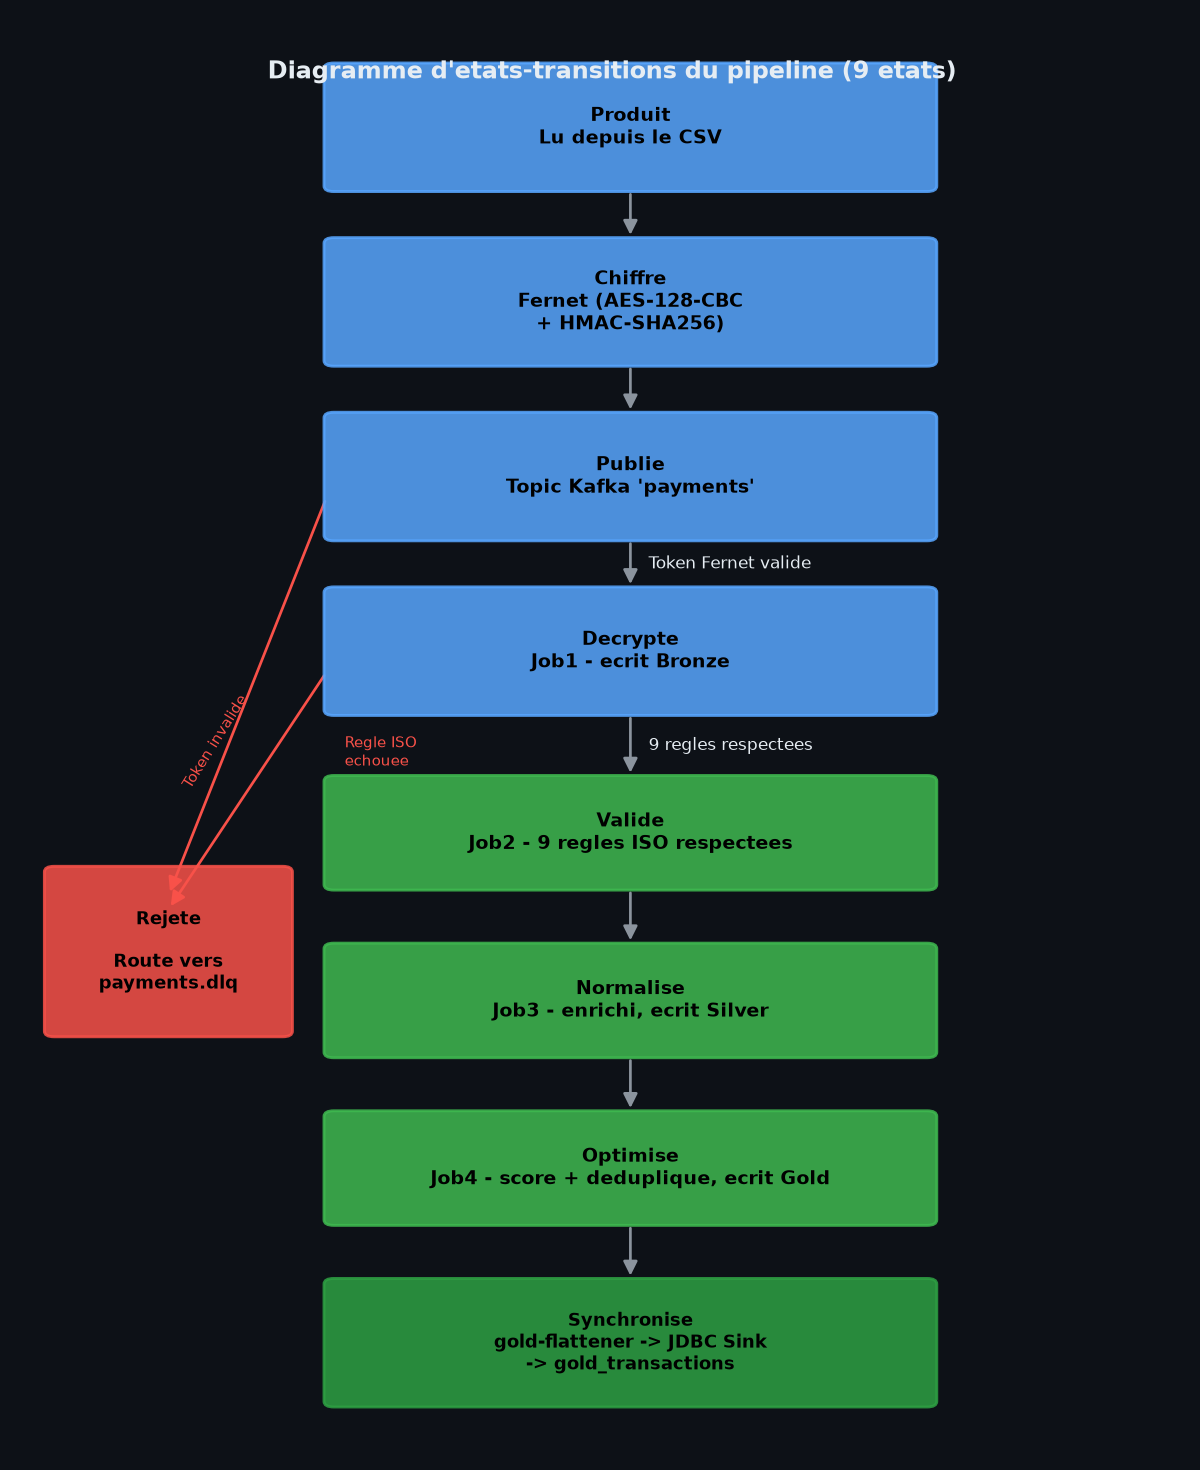
\includegraphics[width=0.85\textwidth]{figures/etats.png}
\caption{Diagramme d'etats-transitions du pipeline (9 etats)}
\label{fig:etats}
\end{figure}

\subsection{Diagramme d'activite}

Le diagramme d'activite (figure \ref{fig:activite}) detaille le flux decisionnel de la
validation des transactions au sein du Job 2. Les 9 regles sont appliquees
sequentiellement ; chaque echec route immediatement la transaction vers
\texttt{payments.dlq} avec un code de rejet machine-readable specifique, sans
poursuivre l'evaluation des regles suivantes.

\begin{figure}[H]
\centering
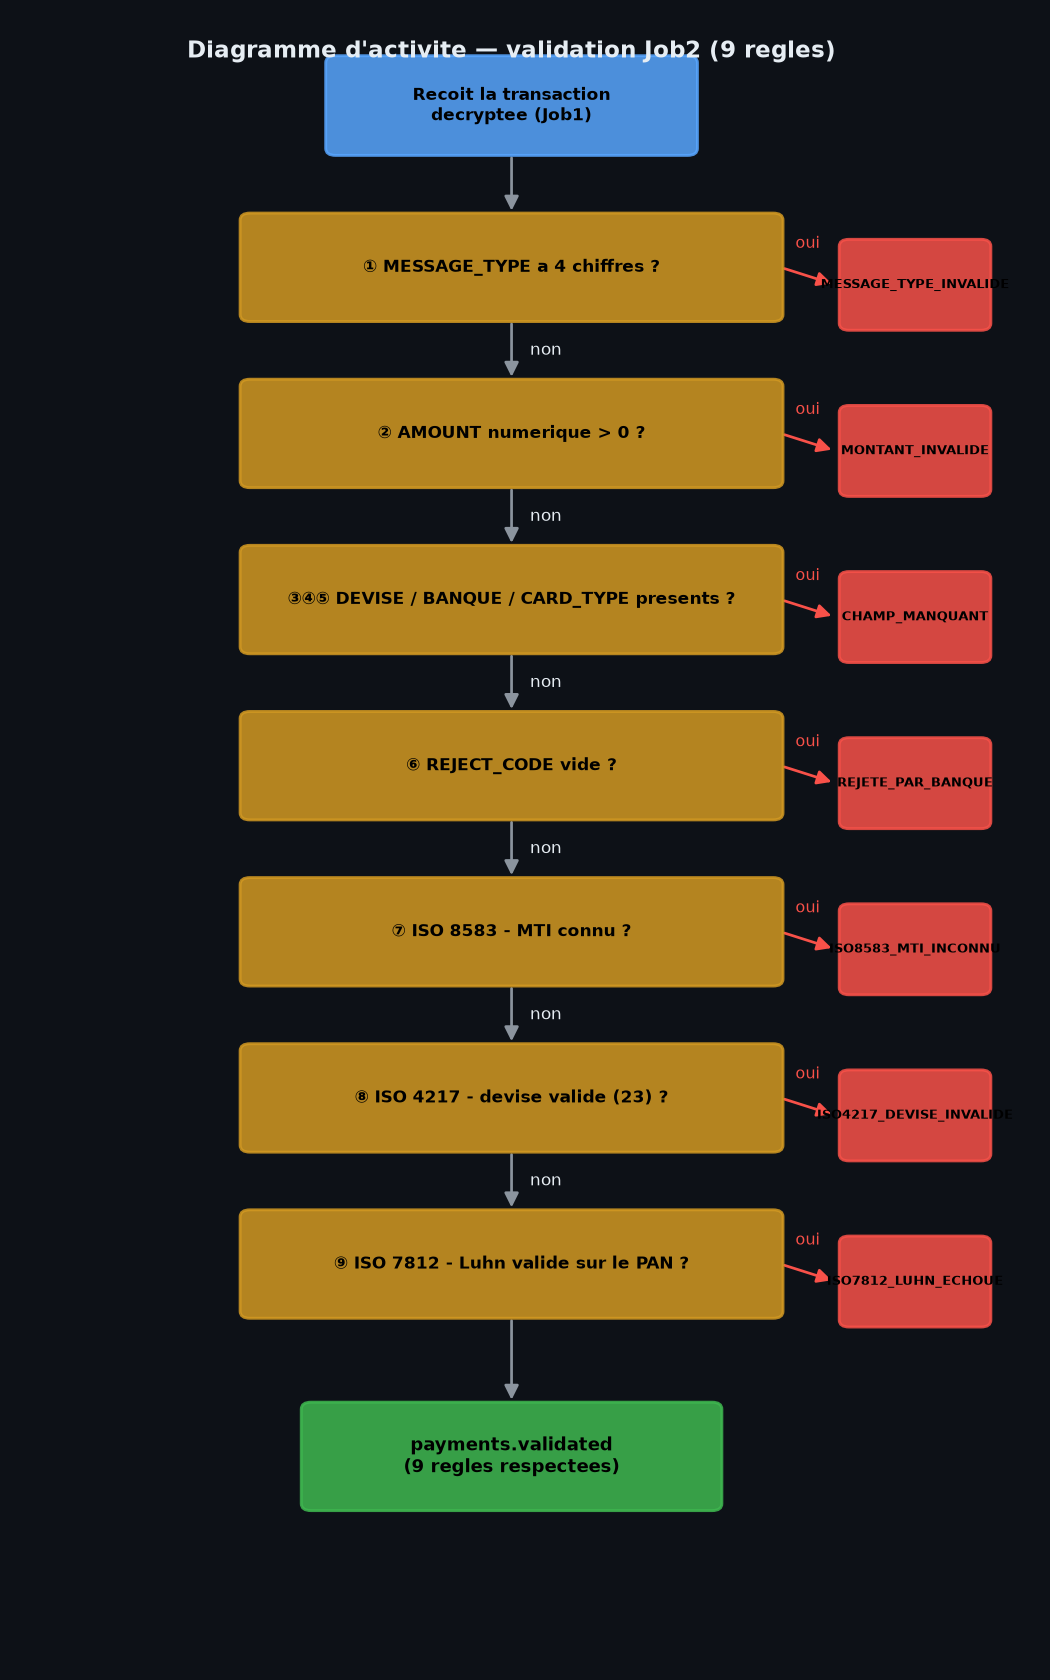
\includegraphics[width=0.75\textwidth]{figures/activite.png}
\caption{Diagramme d'activite --- validation Job2 (9 regles)}
\label{fig:activite}
\end{figure}

\section{Modelisation statique}
\label{sec:statique}

\subsection{Diagramme de classes}

Le diagramme de classes modelise la structure statique des entites principales du
systeme et leurs relations, depuis la reception du message Kafka jusqu'au stockage en
couche Gold.

\textbf{Description des classes principales :}
\begin{itemize}
    \item \textbf{FlinkJob} : classe abstraite representant un job Flink generique,
    definissant les attributs communs (\texttt{jobId}, \texttt{sourceTopic},
    \texttt{sinkTopic}, \texttt{checkpointIntervalMs}) et les methodes
    \texttt{open()}, \texttt{process\_element()} et \texttt{execute()}. Quatre classes
    concretes en heritent : \texttt{DecryptJob}, \texttt{ValidateJob},
    \texttt{NormalizeJob} et \texttt{OptimizeJob},
    \item \textbf{KafkaEnvelope} : represente le message Kafka publie par le
    producteur (\texttt{eventId}, \texttt{table}, \texttt{operation},
    \texttt{payload}, \texttt{timestamp}),
    \item \textbf{Transaction} : donnees de transaction apres dechiffrement par le
    Job 1 (\texttt{MESSAGE\_TYPE}, \texttt{TRANSACTION\_AMOUNT},
    \texttt{TRANSACTION\_CURRENCY}, \texttt{ISSUING\_BANK}, \texttt{CARD\_TYPE},
    \texttt{AUTHORIZATION\_CODE}, \texttt{REJECT\_CODE}, \texttt{PRODUCT\_CODE}),
    \item \textbf{ValidationResult} : resultat de la validation par le Job 2
    (\texttt{status}, \texttt{rejectReason}, \texttt{validatedAt}),
    \item \textbf{NormalizedTransaction} : etend \texttt{Transaction} avec les
    donnees normalisees par le Job 3,
    \item \textbf{EnrichedTransaction} : etend \texttt{NormalizedTransaction} avec
    \texttt{paymentChannel}, \texttt{riskScore} et \texttt{optimizedAt},
    \item \textbf{DLQRecord} : enregistrement rejete (\texttt{errorCode},
    \texttt{errorType}, \texttt{sourceJob}) --- le payload chiffre original n'y figure
    jamais,
    \item \textbf{MedallionLayer} : couche de stockage MinIO (Bronze, Silver ou Gold).
\end{itemize}

\begin{figure}[H]
\centering
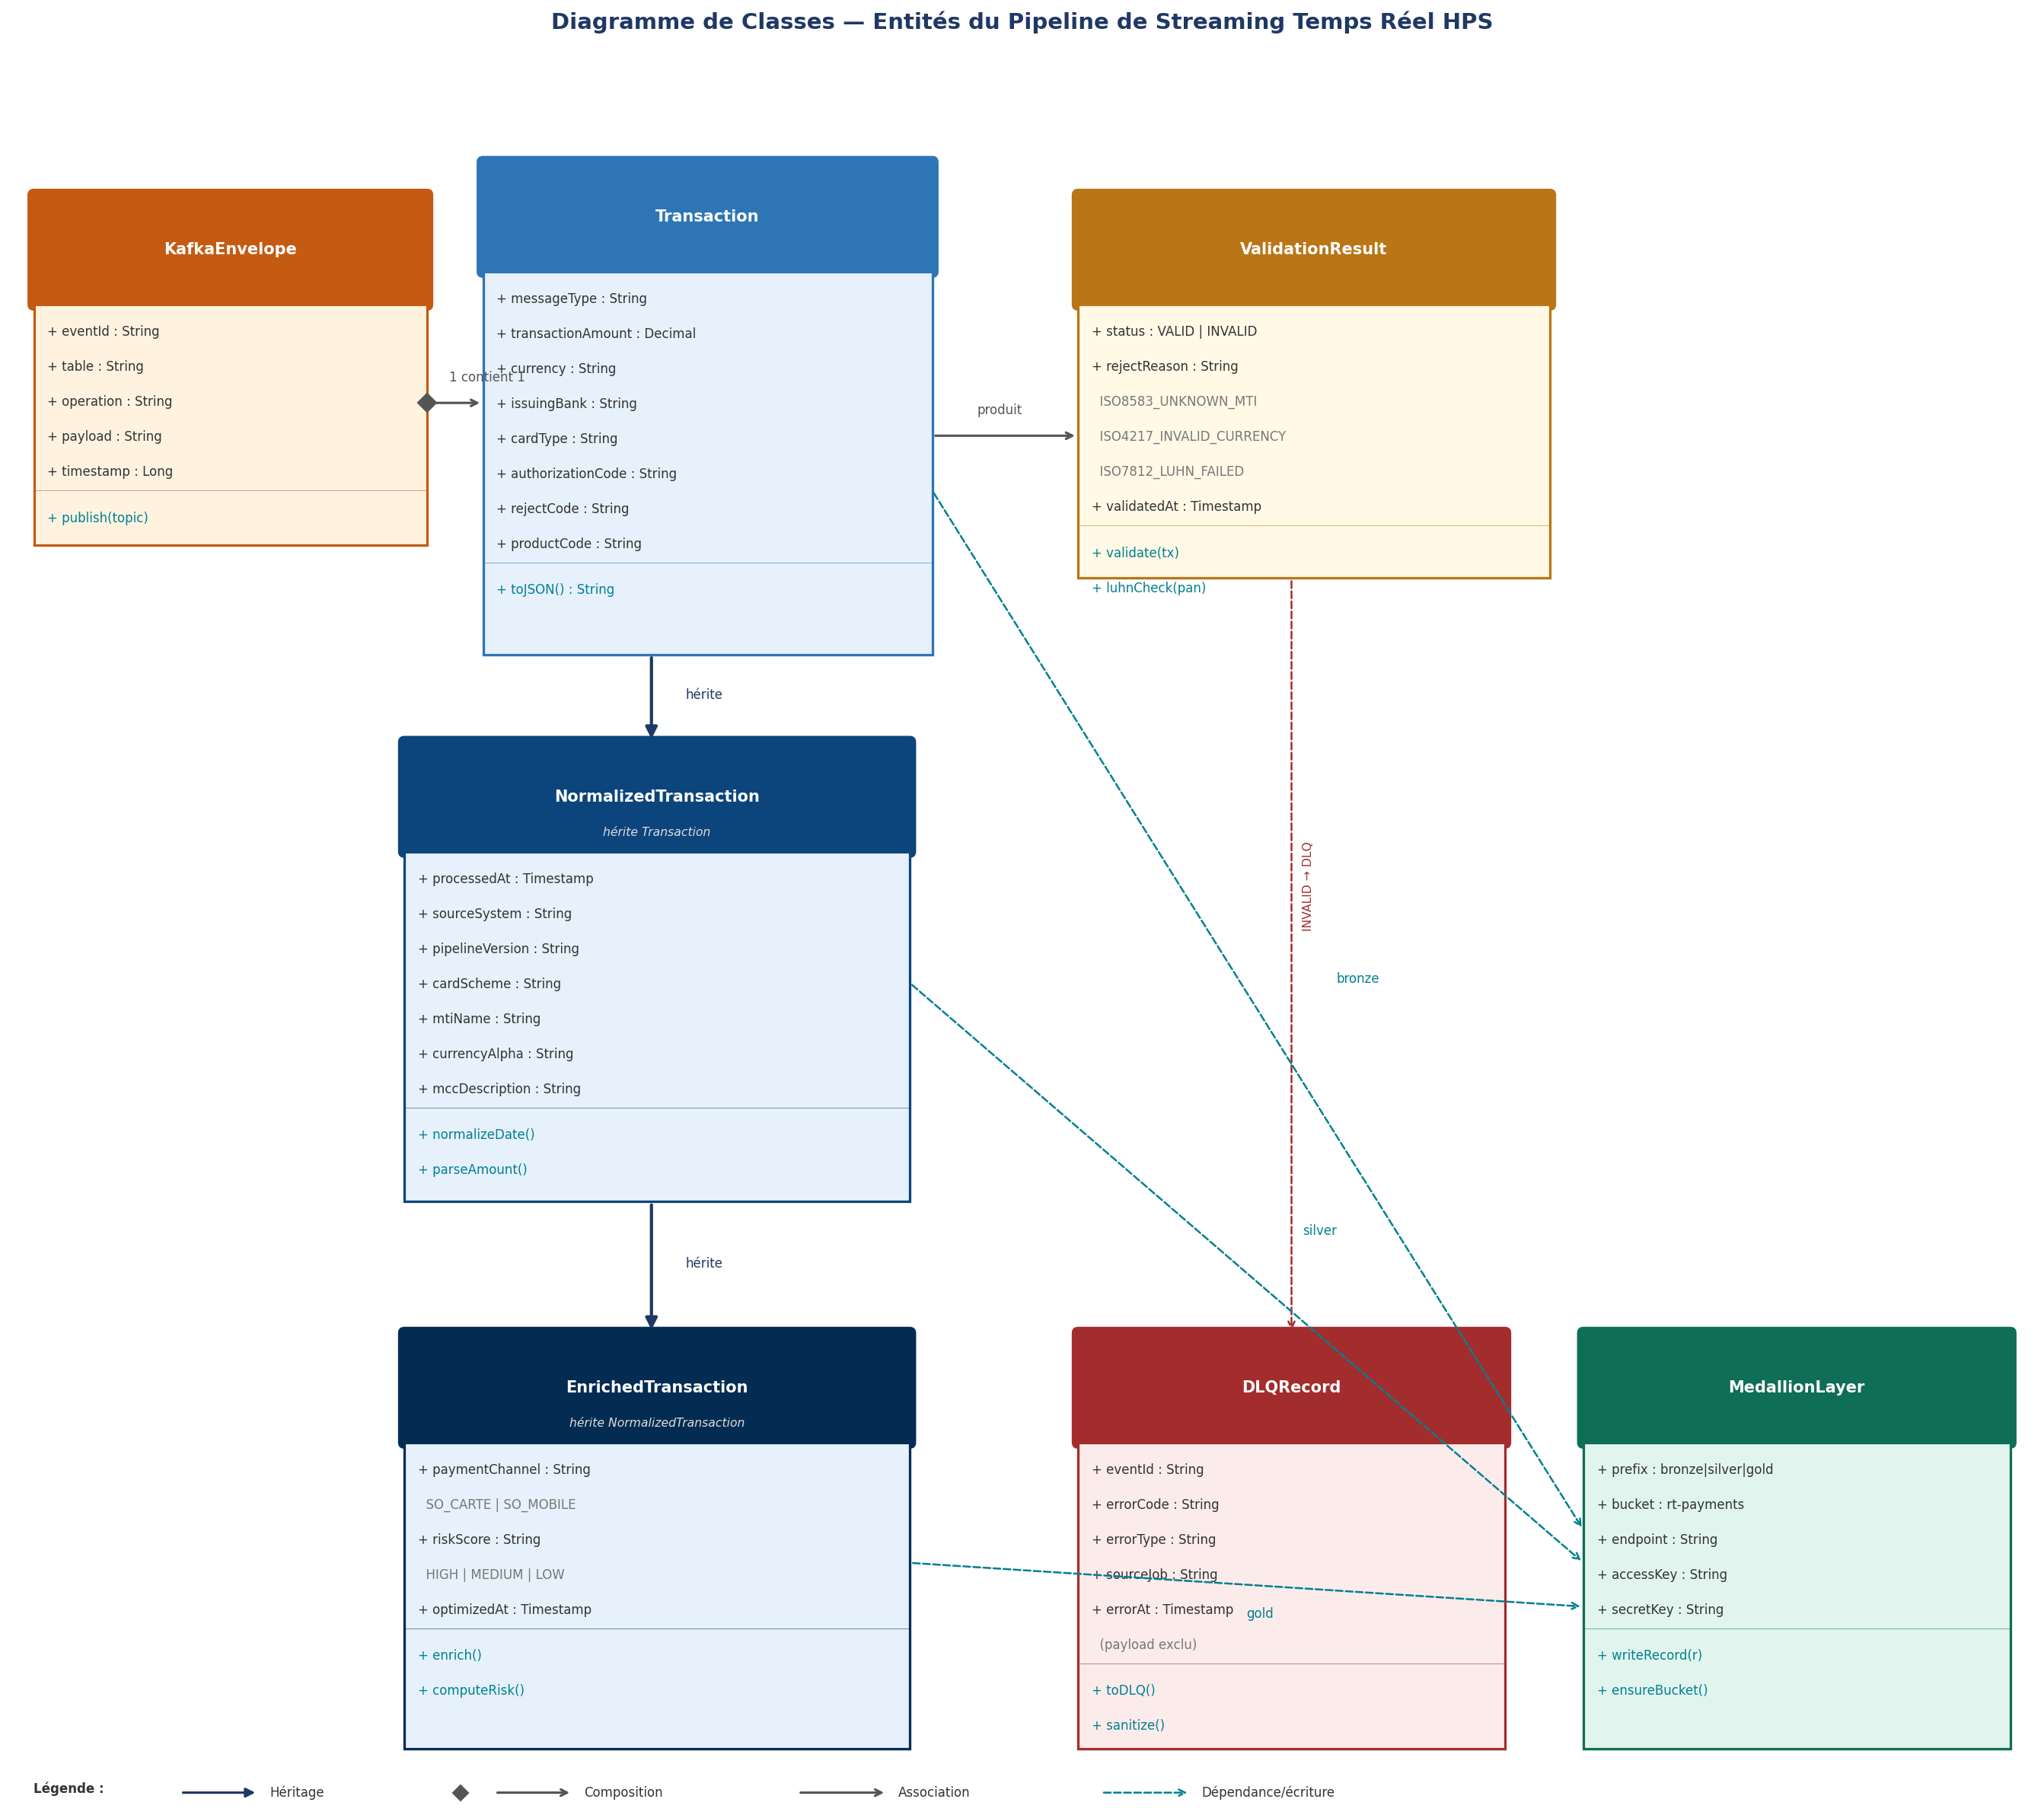
\includegraphics[width=\textwidth]{figures/diagrammeClasses.png}
\caption{Diagramme de classes --- entites du pipeline de streaming temps reel}
\label{fig:classes}
\end{figure}

\subsection{Modele relationnel}

Contrairement a une architecture en etoile multi-tables, le modele relationnel retenu
pour la persistance finale est volontairement \textbf{plat} : une unique table
\texttt{gold\_transactions}, sans tables de dimension, alimentee directement par le
flux \texttt{payments.gold.flat} produit par \texttt{gold-flattener}. Ce choix
simplifie l'integration avec le connecteur Kafka Connect JDBC Sink, qui ecrit chaque
enregistrement en mode \textit{upsert} sur la cle primaire \texttt{authorization\_code}.

\begin{figure}[H]
\centering
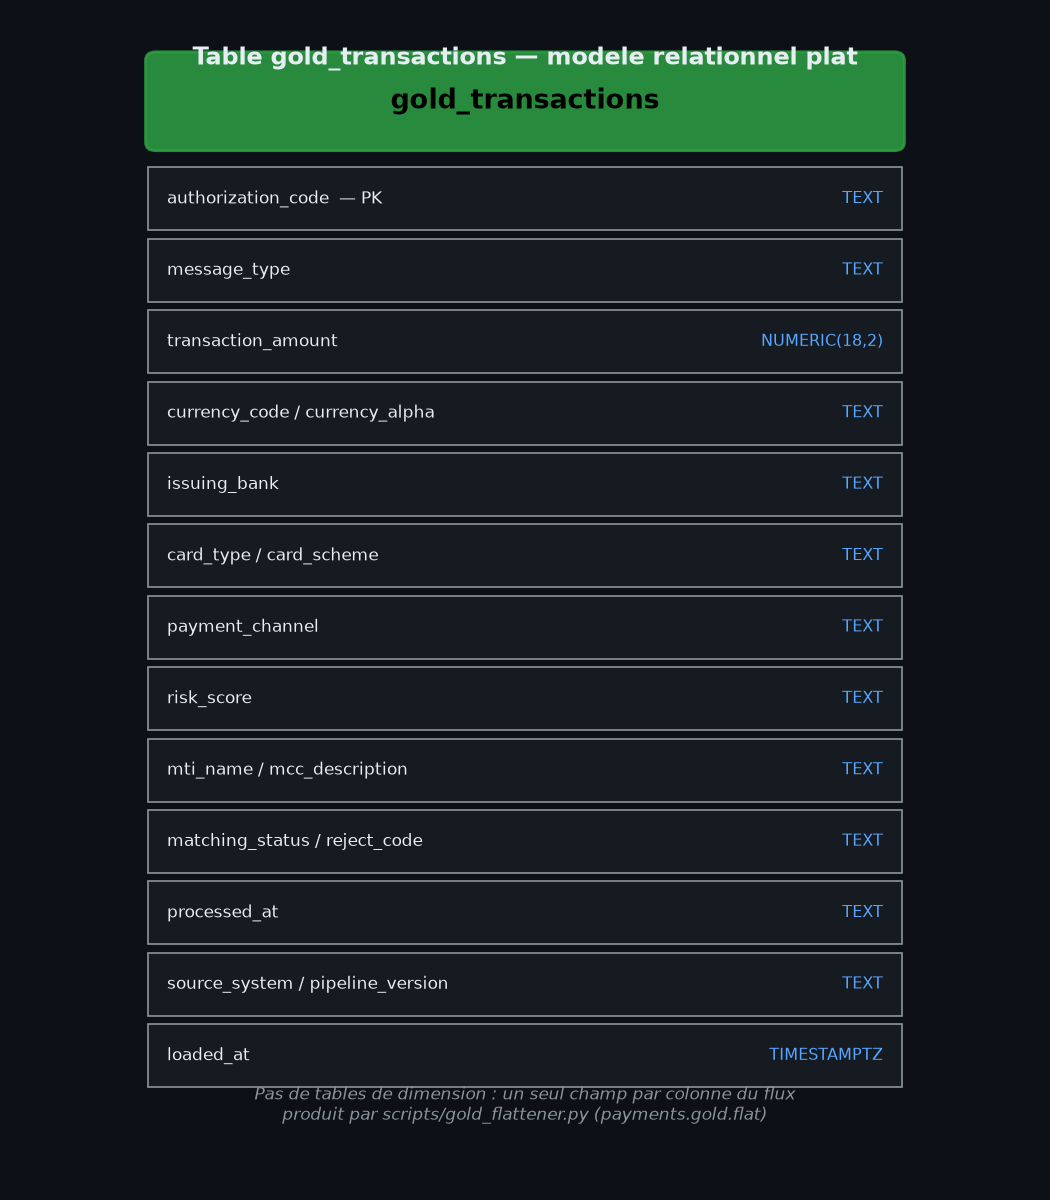
\includegraphics[width=0.7\textwidth]{figures/star_schema.png}
\caption{Table gold\_transactions --- modele relationnel plat}
\label{fig:modele-relationnel}
\end{figure}

\subsection{Dictionnaire de donnees}

Le tableau \ref{tab:dictionnaire} detaille l'ensemble des champs de la table
\texttt{gold\_transactions}.

\begin{longtable}{@{} l l p{6.2cm} @{}}
\toprule
\textbf{Champ} & \textbf{Type} & \textbf{Description} \\
\midrule
\endhead
\texttt{authorization\_code} & \texttt{TEXT} (PK) & Code d'autorisation, identifiant unique de la transaction \\
\texttt{message\_type} & \texttt{TEXT} & Type de message ISO 8583 (MTI) \\
\texttt{transaction\_amount} & \texttt{NUMERIC(18,2)} & Montant de la transaction \\
\texttt{currency\_code} & \texttt{TEXT} & Code devise numerique ISO 4217 \\
\texttt{currency\_alpha} & \texttt{TEXT} & Code devise alphabetique (ex. MAD, EUR) \\
\texttt{issuing\_bank} & \texttt{TEXT} & Banque emettrice de la carte \\
\texttt{card\_type} & \texttt{TEXT} & Type de carte \\
\texttt{card\_scheme} & \texttt{TEXT} & Reseau de la carte (VISA, MASTERCARD, ...) \\
\texttt{payment\_channel} & \texttt{TEXT} & Canal de paiement (\texttt{SO\_CARTE} / \texttt{SO\_MOBILE}) \\
\texttt{risk\_score} & \texttt{TEXT} & Score de risque (\texttt{HIGH}/\texttt{MEDIUM}/\texttt{LOW}) \\
\texttt{mti\_name} & \texttt{TEXT} & Libelle du MTI ISO 8583 \\
\texttt{mcc\_description} & \texttt{TEXT} & Description du code marchand (MCC) \\
\texttt{matching\_status} & \texttt{TEXT} & Statut de rapprochement \\
\texttt{reject\_code} & \texttt{TEXT} & Code de rejet eventuel transmis par la banque \\
\texttt{processed\_at} & \texttt{TEXT} & Horodatage de traitement (ISO 8601) \\
\texttt{source\_system} & \texttt{TEXT} & Systeme source de la transaction \\
\texttt{pipeline\_version} & \texttt{TEXT} & Version du pipeline ayant produit l'enregistrement \\
\texttt{loaded\_at} & \texttt{TIMESTAMPTZ} & Horodatage d'insertion dans PostgreSQL (defaut \texttt{now()}) \\
\bottomrule
\caption{Dictionnaire de donnees --- table \texttt{gold\_transactions}}
\label{tab:dictionnaire}
\end{longtable}

\section{Architecture de l'application}
\label{sec:architecture}

\subsection{Architecture logicielle --- diagramme de composants}

La figure \ref{fig:components} presente le diagramme de composants du pipeline,
depuis la production des transactions jusqu'a leur persistance finale et leur
exposition dans les tableaux de bord de supervision.

\begin{figure}[H]
\centering
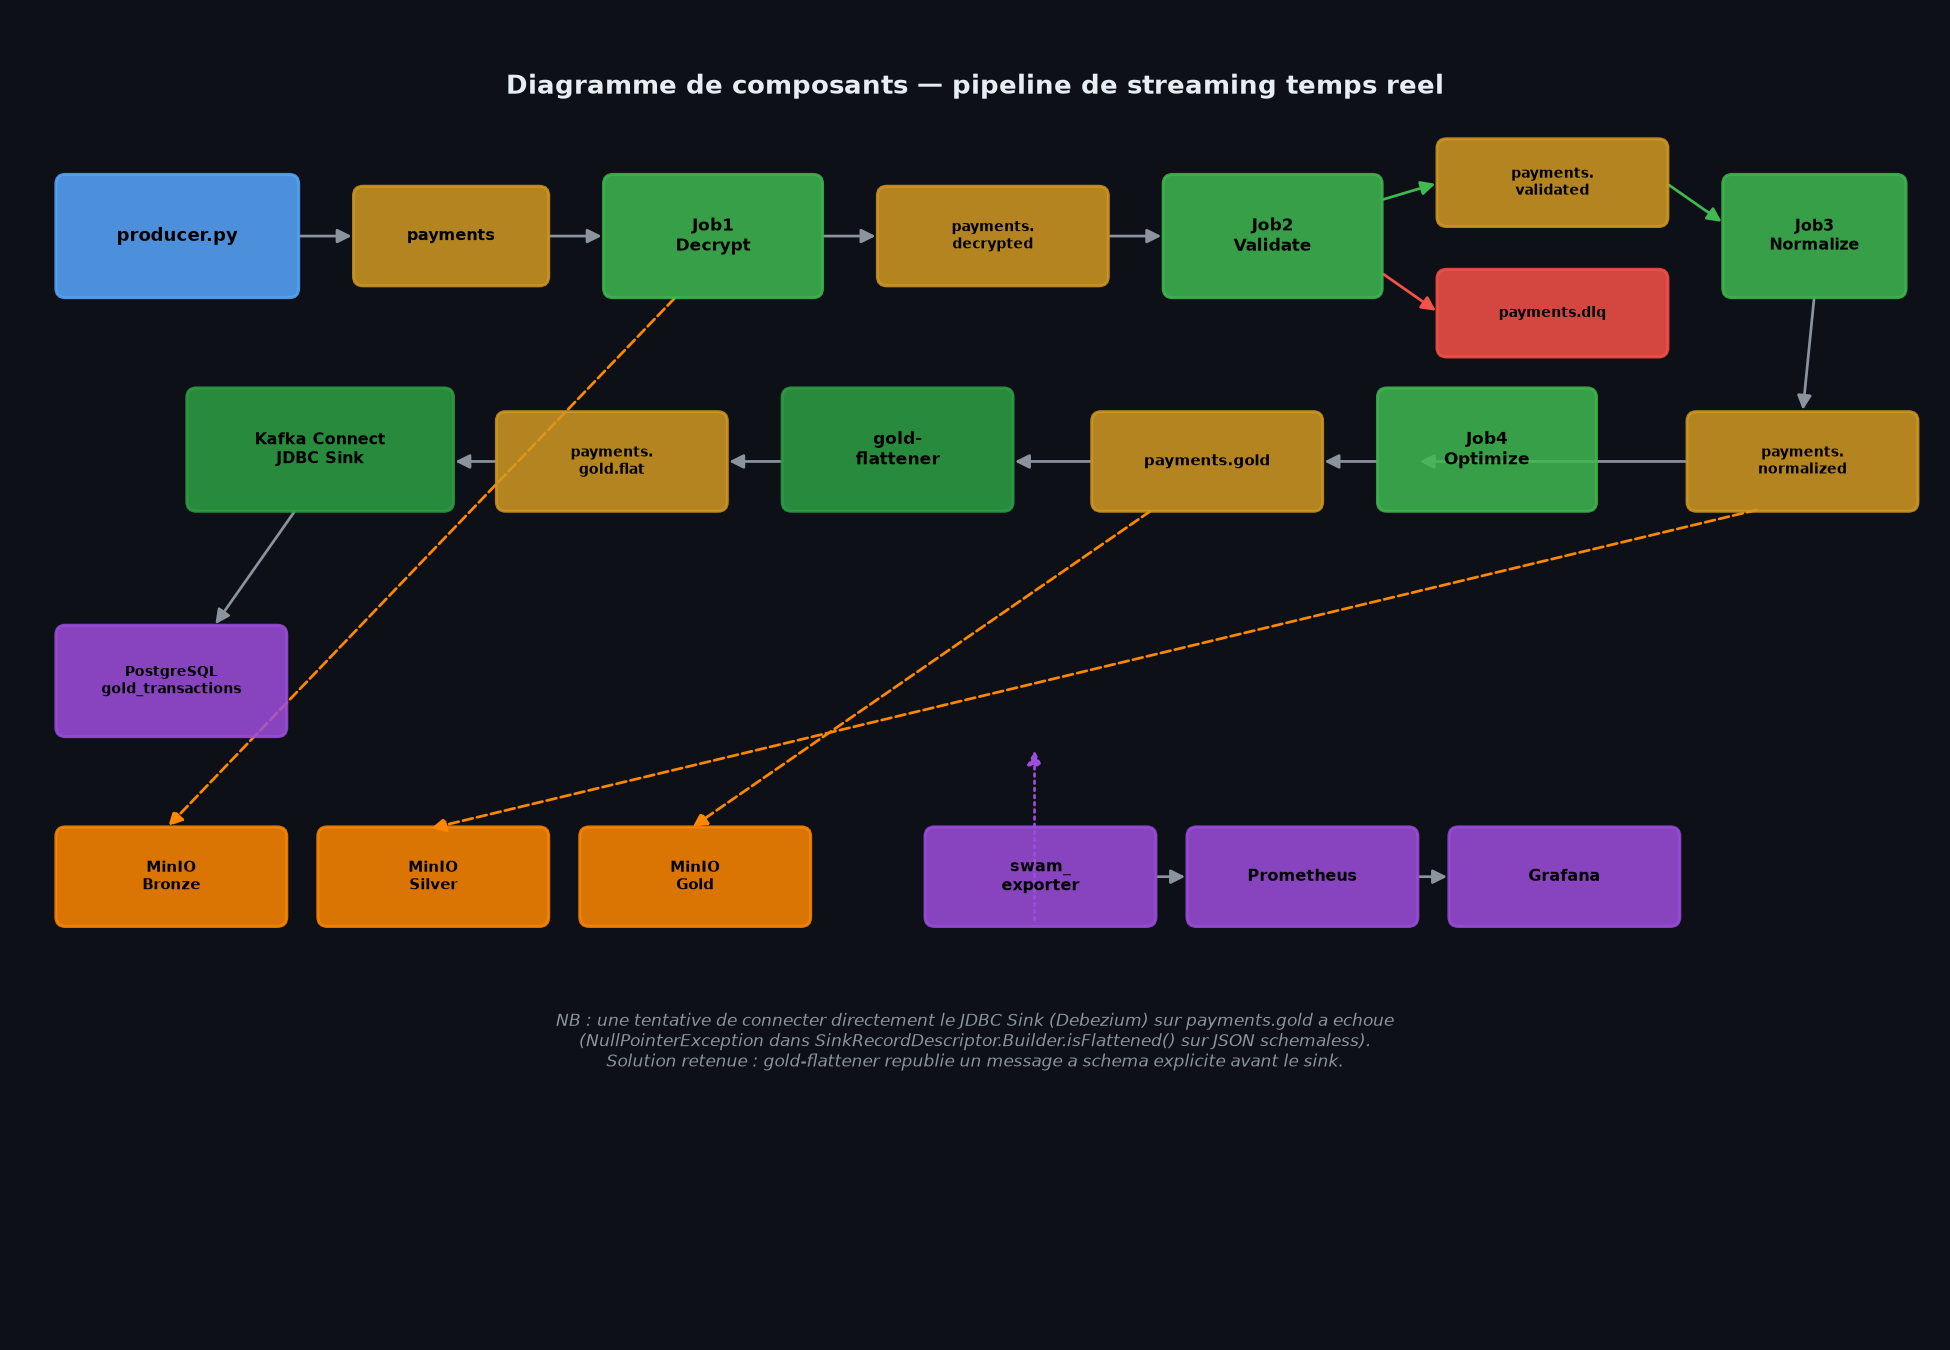
\includegraphics[width=\textwidth]{figures/components.png}
\caption{Diagramme de composants --- pipeline de streaming temps reel}
\label{fig:components}
\end{figure}

Le flux global s'organise ainsi : le \textbf{producteur} publie les transactions
chiffrees dans Kafka (topic \texttt{payments}) ; les quatre \textbf{jobs Flink}
traitent successivement chaque message (decryptage, validation, normalisation,
optimisation), en ecrivant respectivement dans les couches \textbf{Bronze},
\textbf{Silver} et \textbf{Gold} de \textbf{MinIO} ; le composant
\textbf{gold-flattener} consomme \texttt{payments.gold} et republie chaque
enregistrement sous forme de message a schema explicite dans
\texttt{payments.gold.flat} ; le connecteur \textbf{Kafka Connect JDBC Sink} insere
enfin chaque enregistrement dans \textbf{PostgreSQL} (\texttt{gold\_transactions}) ;
en parallele, l'\textbf{exporteur de metriques} interroge Kafka, MinIO et PostgreSQL
pour alimenter \textbf{Prometheus}, lui-meme visualise par \textbf{Grafana}.

Il convient de souligner qu'une premiere tentative a consiste a connecter directement
le connecteur Kafka Connect JDBC Sink (Debezium) sur le topic \texttt{payments.gold}.
Cette approche s'est heurtee a une exception \texttt{NullPointerException} levee par
\texttt{SinkRecordDescriptor.Builder.isFlattened()}, le connecteur exigeant un schema
Kafka Connect explicite (\texttt{schema} + \texttt{payload}) alors que les messages
\texttt{payments.gold} sont publies en JSON schemaless. La solution retenue ---
introduire le composant intermediaire \textbf{gold-flattener} qui republie chaque
enregistrement avec un schema explicite --- a permis de resoudre ce blocage sans
modifier le comportement des jobs Flink existants.

\subsection{Architecture materielle --- diagramme de deploiement}

L'ensemble du systeme est deploye sur un cluster \textbf{Minikube} (6 vCPU, 6~Go de
RAM, pilote Docker), organise en cinq namespaces Kubernetes isoles :

\begin{itemize}
    \item \texttt{kafka} : cluster Kafka en mode KRaft (operateur Strimzi), topics et
    operateurs associes,
    \item \texttt{flink} : JobManager et TaskManagers executant les quatre jobs
    PyFlink,
    \item \texttt{minio} : stockage objet S3-compatible (architecture Medallion),
    \item \texttt{kafka-connect} : worker Kafka Connect, connecteurs source et sink,
    bases PostgreSQL et composant \texttt{gold-flattener},
    \item \texttt{monitoring} : Prometheus, Grafana et \texttt{kube-state-metrics}.
\end{itemize}

L'ensemble de cette infrastructure est provisionne de maniere reproductible via
\textbf{Terraform}, qui orchestre les Helm releases (Strimzi, MinIO), les namespaces,
et les ressources applicatives (ConfigMaps, Deployments) via le pattern
\texttt{null\_resource} associe a des appels \texttt{kubectl apply} idempotents pour
les ressources non nativement supportees par le provider Kubernetes Terraform.

\conclusionchapitre

Ce chapitre a detaille la conception du systeme sous ses trois angles --- dynamique,
statique et architectural --- en justifiant notamment le choix d'un modele
relationnel plat et l'introduction du composant \texttt{gold-flattener} pour
contourner une limitation technique du connecteur JDBC Sink. Le chapitre suivant
presente la realisation effective de ce systeme.
